\documentclass[10pt]{article}

\usepackage{times,fullpage,graphicx,amsmath, subfigure}
\usepackage[pdfborder={0 0 0}]{hyperref}

\title{Methpipe Manual}
\author{Qiang Song \and Michael Kessler \and Fang Fang \and Jenny Qu \and
Tyler Garvin \and Andrew Smith}

\newcommand{\meth}{\texttt{methpipe}}

%%%%
%%%% NOTE: use the following appropriately so that we can change the
%%%% individual types later.
%%%%
%%
%% For program names
\newcommand{\prog}[1]{\texttt{#1}}
%% For file names
\newcommand{\fn}[1]{\texttt{#1}}
%% For literals
\newcommand{\lit}[1]{\texttt{#1}}
%% For program options
\newcommand{\op}[1]{\texttt{#1}}

\begin{document}

\maketitle

The \meth{} software package is a comprehensive pipeline and set of
tools for analyzing whole genome bisulfite sequencing data
(BS-seq). This manual explains the stages in our pipeline, how to use
the analysis tools, and how to modify the pipeline for your specific
context.

\section{Assumptions}

Our pipeline was designed to run in a cluster computing context, with
many processing nodes available, and a job submission system like PBS
or SGE. Much of this analysis is computationally intensive. We assume
that individual nodes will have several GB of memory available for
processing. Typically the data we deal with amounts to a minimum of
100GB for a mammalian methylome at 10x coverage. Intermediate files
may cause this amount to more than double during execution of the
pipeline, and likely at the end of the pipeline the total size of
files will amount to almost double the size of the raw data.

Users are assumed to be quite familiar with UNIX/Linux and related
concepts ({\em e.g.} building software from source, using the command
line, shell environment variables, etc.).

It is also critical that users are familiary with BS-seq experiments,
especially the bisulfite conversion reaction, and how this affects
what we observe in the sequenced reads. Especially if paired-end
sequencing is used. If you do not understand these concepts, you will
likely run into major problems trying to customize our pipeline.

\section{Methylome construction}

\subsection{Mapping reads}
\label{sec:mapping}

% \begin{description}
% \item[rmapbs.cpp]
% This program takes fastq file as input and output mapped read file
% \end{description}

During bisulfite treatment, unmethylated cytosines in the original DNA
sequences are converted to uracils, which are then incorporated as
thymines (T) during PCR amplification. These PCR products are referred
to as T-rich sequences as a result of their high thymine
constitution. With paired-end sequencing experiments, the compliments
of these T-rich sequences are also sequenced.  These complimentary
sequences have high adenosine (A) consitution (A is the complimentary
base pair of T), and are referred to as A-rich sequences. Mapping
consists of finding sequence similary, based on context specific
criteria, between these short sequences, or reads, and a homologous
(orthologous?) reference genome.  When mapping T-rich reads to the
reference genome, either a cytosine (C) or a thymine (T) in a read is
considered a valid match for a cytosine in the reference genome. For
A-rich reads, an adenine or a guanine is considered a valid match for
a guanine in the reference genome. The mapping of reads to the
reference genome by \prog{rmapbs} is described below. If you choose
to map reads with a different tool, make sure that your post-mapping
files are approrpiately formatted for the next components of the
\meth{} pipeline (necessary file formats for each step are covered in
the corresponding sections).  The deault behavior of rmapbs is to
assume that reads are T-rich and map accordingly. To change the
mapping to suit A-rich reads, add the \op{-A} option.

\paragraph{Input and output file formats:} We assume that the original
data is a set of sequenced read files, typically as produced by
Illumina sequencing. These are FASTQ format files, and can be quite
large. After the reads are mapped, these files are not used by our
pipeline.

The mapped reads files (\fn{*.mr} suffix) that result from the previous
steps should consist of eight columns of data. The first six columns
are the traditional components of a BED file (chromosome, start, end,
name, score, strand), while the last two columns consist of sequence
and quality scores respectively. These mapped reads files will be the
input files for the following two \meth{} components, \prog{bsrate}
and \prog{methcounts}.

\paragraph{Partitioning reads for mapping using a cluster:} Mapping
reads often takes a while, and mapping reads from BS-seq takes longer.
Because of how \prog{rmapbs} works, dividing the set of reads to be
mapped into $k$ equal sized smaller reads files, and mapping these all
simultaneously on a cluster, will make the mapping finish about $k$
times faster. I will typically map 3M reads at a time, and this takes
at most 1.5GB of memory for the human genome and with 100nt reads. The
unix \prog{split} command is good for dividing the reads into smaller
parts. The following BASH commands will take a directory named
\fn{reads} containing Illumina sequenced reads files, and split
them into files containing at most 3M reads:
\begin{verbatim}
$ mkdir reads_split
$ for i in reads/*.txt; do \
    split -a 3 -d -l 12000000 ${i} reads_split/$(basename $i); done
\end{verbatim}
Notice that the number of lines per split file is 12M, since we want
3M reads, and there are 4 lines per read. If you split the reads like
this, you will need to ``unsplit'' them after the mapping is done. Not a
problem, just use the \prog{cat} command (example will be given
below).

\paragraph{Sequencing adaptors:} These are a problem in any sequencing
experiment with short fragments relative to the lengths of reads.  The
\prog{cutadapt} program does a fine job removing adaptors. If you plan
to use \prog{rmapbs} after removing the adaptors, then you will need to
replace the parts of the reads that get removed with \lit{N} characters.
These will not influence the mapping, because they will be treated as
wildcard characters by \prog{rmapbs}, but reads are currently required
to be the same length in \prog{rmapbs}.

You can also have \prog{rmapbs} cut the adaptors for you. All you need
to do is provide the adaptor sequence on the command
line. \prog{rmapbs} will only cut the adaptor if it sees at least 10nt
of the adaptor, and the rest of the adaptor sequence extending towards
the 3' end of the read. This will work for both ends of paired-end
reads. The situation of adaptor concatamers, where the adaptor begins
immediately at the beginning of the read, may not be handled well.

\paragraph{Single-end reads:}
When working with data from a single-end sequencing experiment, you
will have T-rich reads only. \prog{rmapbs} expects T-rich reads as a
default and so you do not have use the \op{-A} option to change mapping
parameters. Execute the following command to map all of your
single-end reads with \prog{rmapbs}.
\begin{verbatim}
$ ./rmapbs -c hg18 -o Human_NHFF.mr Human_NHFF.fastq
\end{verbatim}

\paragraph{Paired-end reads:}
When working with data from a paired-end sequencing experiment, you
will have T-rich and A-rich reads. T-rich reads are often kept in
files labeled with an ``\_1'' and A-rich reads are often kept in files
labeled with an ``\_2''. We will follow this convention throught the
manual and strongly suggest that you do the same. T-rich reads are
sometimes referred to as $5^{\prime}$ reads or mates 1 and A-rich
reads are sometimes referred to $3^{\prime}$ reads or mates 2; we will
stick with T-rich and A-rich. \prog{rmapbs} expects T-rich reads as a
default and so for paired-end sequencing data, you must run
\prog{rmapbs} twice; once for T-rich reads and once for A-rich
reads. Execute the following commands to map of your paired-end reads
with \prog{rmapbs}; one command for T-rich reads, and one for A-rich
reads.
\begin{verbatim}
$ ./rmapbs -c hg18 -o Human_ESC_1.mr Human_ESC_1.fastq
\end{verbatim}
An example command for the second end (previously named like
\fn{s\_1\_2\_sequence.txt} from Illumina), which will contain all
A-rich reads:
\begin{verbatim}
$ ./rmapbs -c hg18 -o Human_ESC_2.mr -A Human_ESC_2.fastq
\end{verbatim}

\paragraph{Merging paired-end reads:}
As previously noted, paired-end sequencing produces both T-rich reads
and A-rich reads. Since methylation is estimated from the counts of Ts
and Cs (that map to C's in the reference genome), and A-rich reads
contain methylation information in the form of A and G counts (that
map to Gs in the reference genome), A-rich reads must turned into
T-rich reads by reverse complimenttion. This allows methylation
information to be derived from the Ts and Cs in the new T-rich reads
that correspond to the As and Gs from the A-rich reads that was
reverse complementated.

A double counting error could arise if overlapping regions exist
between any two mates. To avoid this error and maintain all other
important information, we replace bases in the overlapping region with
Ns in one of the two mates. Reverse-complemention of A-rich reads (and
switching the strand to which they mapped), and masking overlapping
regions, are done by the program \prog{clipmates}. This tool works on
mapped reads files that been sorted by read id (read name). The
following command is an example of how to sort your mapped reads files
with the Unix \prog{sort} command before inputting them into
\prog{clipmates}.
\begin{verbatim}
$ sort -k 4,4 -o Human_ESC_1.mr.sorted Human_ESC_1.mr
$ sort -k 4,4 -o Human_ESC_2.mr.sorted Human_ESC_2.mr
\end{verbatim}
The names of corresponding mates must only differ by the last
character (which should be a 1 for T-rich reads and 2 for A-rich
reads). If mates exist and are mapped correctly (to the same
chromosome, to correct strands, with correct orientation) within a
certain distance from each other (as specified by the \op{-L} option),
then the mates are combined into a single read, referred to as a
fragment, with Ns filling any existing gaps between mates. If mates
could not be matched, then each mate is present in the output
file. \prog{clipmates} takes two input files in mapped reads format:
one with T-rich mreads (\op{-T} option) and the other with A-rich
reads (\op{-A} option). Execute the following command to run the
\prog{clipmates} component of \meth{} on T-rich and A-rich reads
(mates 1 and 2).
\begin{verbatim}
$ ./clipmates -S Human_ESC.clipstats -o Human_ESC.mr \
              -T Human_ESC_1.mr.name_sorted -A Human_ESC_2.mr.name_sorted
\end{verbatim}

% \noindent OPTIONS:
% \begin{itemize}
% \item
% \textbf{-v}, \textbf{-verbose} : be verbose; print more run info
% \item
% \textbf{-L}, \textbf{-max-frag}  \textless integer\textgreater : maximum length between mates (default: 1000)
% \item
% \textbf{-S}, \textbf{-out\_stat} \textless string\textgreater : clipmates statistics output file name
% \item
% \textbf{-T}, \textbf{-t-rich} \textless string\textgreater : input file with mates 1 (T-rich mates)
% \item
% \textbf{-A}, \textbf{-a-rich} \textless string\textgreater : input file with mates 2 (A-rich mates)
% \item
% \textbf{-s},\textbf{-suff} \textless integer|textgreater : read name suffix length (default: 1)
% \item
% \textbf{-o}, \textbf{-outfile} \textless string\textgreater : output file name
% \end{itemize}

% \noindent NPUT: Two files in Maped Reads format: one with T-rich reads(mate 1) and the other with A-rich reads (mate 2).

% \noindent OUTPUT: mapped reads format with combined DNA fragments and single mates. File with
% paired-end mapping statistics has self-explanatory content.


\subsection{Merging libraries and removing duplicates}
\label{sec:mapping}

Before calculating methylation level, you should now remove read
duplicates, or reads that were mapped to the same genomic
location. These reads are most likely the results of PCR
over-amplication rather than true representations of distinct DNA
molecules. The program \prog{duplicate-remover} can be used to remove
such duplicates. It collects reads and fragments mapped to the same
genomic location (start or end), and chooses a random one to be the
representative of the original DNA sequence. Since sequencing can run
for variable lengths of time (leading to different length reads), we
must sort reads by the position of the side where sequenceing starts
in order to find duplicates. This is always the 5' side, which for +
strand reads is their start positions and for - strand reads is the
end positions. Therefore, two separte sorts and removals of duplicates
must be done; one on + strand reads while sorting on start positions,
and one on - strand reads while sorting on end position. The \op{-B}
option of \prog{duplicate-remover} ignores + reads and tells the
program that reads are sorted by end position. To remove read
duplicates, follow the following steps (examples are provided below):
(1) sort reads by start position (chrom, start, end, strand), (2)
merge files with reads that came from the same DNA library (and
therefore underwent the same PCR) (3) run \prog{duplicate-remover} to
remove read duplicates mapping to the same start positions, (4) sort
reads by end position (chrom, end, start, strand), and (5) run
\prog{duplicate-remover} with option \op{-B} to remove duplicates
mapping to the same end positions.

\begin{sloppypar}
First, sort reads by start position (chrom, start, end,
strand). Remember, for paired-end reads, use the output from climpates
while working through the following steps:
\begin{verbatim}
$ sort -k 1,1 -k 2,2g -k 3,3g -k 6,6 \
       -o Human_ESC.mr.sorted_start Human_ESC.mr
$ sort -k 1,1 -k 2,2g -k 3,3g -k 6,6 \
       -o Human_NHFF.mr.sorted_start Human_NHFF.mr
\end{verbatim}
If at any point during the pipeline you split your files into smaller
files due to size limitations, you should now merge all these split
reads files back into one complete file. We recommend that you do this
using \op{-m} option of the Unix command \prog{sort}. The following
command is an example of how to merge three such files with the
assumption that these files were labled with a 1, 2 or 3 respectively.
\begin{verbatim}
$ sort -m -k 1,1 -k 2,2g -k 6,6 -k 3,3g \
       -o Human_ESC.mr.sorted_start_merged \
       Human_ESC_1.mr.sorted_start \
       Human_ESC_2.mr.sorted_start \
       Human_ESC_3.mr.sorted_start
$ sort -m -k 1,1 -k 2,2g -k 6,6 -k 3,3g \
       -o Human_NHFF.mr.sorted_start_merged \
       Human_NHFF_1.mr.sorted_start \
       Human_NHFF_2.mr.sorted_start \
       Human_NHFF_3.mr.sorted_start
\end{verbatim}
Execute the following command to remove read duplicates sharing the
same start position by running the  \prog{duplicate-remover} component
of \meth{}:
\begin{verbatim}
$ ./duplicate-remover -S Human_ESC_dremove_start_stat.txt \
                      -o Human_ESC_dremove_start.mr Human_ESC_sorted_start.mr
$ ./duplicate-remover -S Human_NHFF_dremove_start_stat.txt \
                      -o Human_NHFF_dremove_start.mr Human_NHFF_sorted_start.mr
\end{verbatim}
Next, sort reads by end position: chrom, end, start, strand.
\begin{verbatim}
$ sort -k 1,1 -k 3,3g -k 2,2g -k 6,6 \
       -o Human_ESC.mr.sorted_end Human_ESC.mr
$ sort -k 1,1 -k 3,3g -k 2,2g -k 6,6 \
       -o Human_NHFF.mr.sorted_end Human_NHFF.mr
\end{verbatim}
Execute the following command to remove read duplicates sharing the
same end position by running the \prog{duplicate-remover} component of
Methpipe.
\begin{verbatim}
$ ./duplicate-remover -S Human_ESC_dremove_start_stat.txt \
                      -o Human_ESC_dremove_end.mr -B Human_ESC_sorted_end.mr
$ ./duplicate-remover -S Human_NHFF_dremove_start_stat.txt \
                      -o Human_NHFF_dremove_end.mr -B Human_NHFF_sorted_end.mr
\end{verbatim}
\end{sloppypar}
\noindent
{\em Need to describe the output format for the stats on the number of
  distinct reads. Also need to describe the reorder tool so that
  re-sorting is not so painful.}

% \noindent OPTIONS:
% \begin{itemize}
% \item
% \textbf{-o} , \textbf{-output} \textless string\textgreater : output file name
% \item
% \textbf{-B}, \textbf{-endpos } : ignore + strand reads, assume sorted order is based on end position, and remove read duplicates sharing the same end position.
% \item
% \textbf{-S}, \textbf{-stats} \textless string\textgreater : Statistics output file name
% \item
% \item
% \textbf{-v}, \textbf{-verbose} : be verbose; print more run info
% \end{itemize}

% \noindent INPUT: A single file in mapped reads format.

% \noindent OUTPUT: The output file is in mapped reads format and statistics file has self-explanatory output.

% \noindent OPTIONS:
% \begin{itemize}
% \item
% \textbf{-o},\textbf{-output} \textless string\textgreater : name of output file (default: stdout)
% \item
% \textbf{-c},\textbf{-chrom}  \textless string\textgreater : name of reference genome file or directory containing reference genome broken into seperate files for each chromosome (requires FASTA format and .fa suffix)
% \item
% \textbf{-s},\textbf{-suffix} \textless string\textgreater : suffix of FASTA files (assumes -c indicates dir)
% \item
% \textbf{-F},\textbf{-Filenames} \textless string\textgreater : file listing names of chromosome files (absolute paths to
% 	chromosome files)
% \item
% \textbf{-S},\textbf{-seeds} \textless integer\textgreater : number of seeds
% \item
% \textbf{-h},\textbf{-hit} \textless integer\textgreater : weight of hit
% \item
% \textbf{-w},\textbf{-width} \textless integer\textgreater : width of the shortest reads in the input
% \item
% \textbf{-m},\textbf{-mismatch} \textless integer\textgreater : maximum allowed mismatches per read
% \item
% \textbf{-a},\textbf{-ambiguous} \textless string\textgreater : file to write names of ambiguously mapped reads
% \item
% \textbf{-M},\textbf{-Max-map} \textless integer\textgreater :  maximum allowed mappings for a read
% \item
% \textbf{-W},\textbf{-wc} : run in wildcard matching mode
% \item
% \textbf{-P},\textbf{-prob} \textless float\textgreater : wildcard cutoff probability
% \item
% \textbf{-Q},\textbf{-qual} : use quality scores (input must be FASTQ)
% \item
% \textbf{-A},\textbf{-ag-wild} : map using A/G bisulfite wildcards (ALWAYS use with mates 2)
% \item
% \textbf{-B},\textbf{-bias} : allow CpG non-conversion to assist
% \item
% \textbf{-f},\textbf{-faster} : use faster seeds (sensitive to 2 mismatches)
% \item
% \textbf{-C},\textbf{-clip}   \textless string\textgreater : clip the specified adaptor
% \item
% \textbf{-v}, \textbf{-verbose} : be verbose; print more run info
% \item
% \textbf{-G},\textbf{-original-output} : use original output format (BED)
% \item
% \textbf{-y},\textbf{-wild-n-mode} : allow N in read to match anything
% \end{itemize}

% \noindent INPUT: Reads are in FASTQ or FASTA format, and references are in FASTA format.

% \noindent OUTPUT: File in mapped reads format. This type of file has eight columns of data consisting of chromosome, start, end,name, score, strand, sequence, and quality score, respectively.

\subsection{Estimating bisulfite conversion rate}
\label{sec:estim-busilf-conv}

Unmethylated cytosines in DNA fragments are converted to uracils by
sodium bisulfite treatment. As these fragments are amplified, the
uracils are converted to thymines and so unmethylated Cs are
ultimately read as Ts (barring error). Despite its high fidelity,
bisulphite conversion of C to T does have some inherent failure rate,
depending on the bisulfite kit used, reagent concentration, time of
treatment, etc., may impact the success rate of the
reaction. Therefore, the bisulfite conversion rate, defined as the
rate at which unmethylated cytosines in the sample appear as Ts in the
sequenced reads, should be measured and should be very high ({\em
  e.g.} $>0.99$) for the experiment to be considered a success.

Measuring the bisulfite conversion rate this way requires some kind of
control set of genomic cytosines not believed to be methylated. Three
options are (1) to spike in some DNA known not to be methylated, such
as a Lambda virus, (2) to use the mitochondrial or chloroplast genomes
which are believed not to be methylated, (3) to use non-CpG cytosines
which are believed to be almost completely unmethylated in most
mammalian cells. In general the procedure is to identify the positions
in reads that correspond to these presumed unmethylated cytosines,
then compute the ratio of C to (C + T) at these positions. If the
bisulfite reaction were perfect, then this ratio should be very close
to 1, and if there is no bisulfite treatment, then this ratio should
be close to 0.

The program \prog{bsrate} will estimate the bisulfite conversion rate
in this way. Assuming method (3) from the above paragraph of measuring
conversion rate at non-CpG cytosines in a mammalian methylome, the
following command will estimate the conversion rate.
\begin{verbatim}
$ ./bsrate -c hg18 -o Human_ESC.bsrate Human_ESC.mr
$ ./bsrate -c hg18 -o Human_NHFF.bsrate Human_NHFF.mr
\end{verbatim}
The \prog{bsrate} program requires that the input be sorted so that
reads mapping to the same chromosome are contiguous. The first several
lines of the output might look like the following:
{\small{%%
\begin{verbatim}
OVERALL CONVERSION RATE = 0.994141
POS CONVERSION RATE = 0.994166  832349
NEG CONVERSION RATE = 0.994116  825919
BASE PTOT  PCONV PRATE   NTOT  NCONV NRATE   BTHTOT BTHCONV BTHRATE ERR ALL    ERRRATE
1    8964  8813  0.9831  9024  8865  0.9823  17988  17678   0.9827  95  18083  0.0052
2    7394  7305  0.9879  7263  7183  0.9889  14657  14488   0.9884  100 14757  0.0067
3    8530  8442  0.9896  8323  8232  0.9890  16853  16674   0.9893  98  16951  0.0057
4    8884  8814  0.9921  8737  8664  0.9916  17621  17478   0.9918  76  17697  0.0042
5    8658  8596  0.9928  8872  8809  0.9929  17530  17405   0.9928  70  17600  0.0039
6    9280  9218  0.9933  9225  9177  0.9948  18505  18395   0.9940  59  18564  0.0031
7    9165  9117  0.9947  9043  8981  0.9931  18208  18098   0.9939  69  18277  0.0037
8    9323  9268  0.9941  9370  9314  0.9940  18693  18582   0.9940  55  18748  0.0029
9    9280  9228  0.9944  9192  9154  0.9958  18472  18382   0.9951  52  18524  0.0028
10   9193  9143  0.9945  9039  8979  0.9933  18232  18122   0.9939  66  18298  0.0036
\end{verbatim}%%
}}

\noindent
The above example is based on a very small number of mapped reads in
order to make the output fit the width of this page.  The first thing
to notice is that the conversion rate is computed separately for each
strand. The information is presented separately because this is often
a good way to see when some problem has occurred in the context of
paired-end reads. If the conversion rate looks significantly different
between the two strands, then we would go back and look for a mistake
that has been made at an earlier stage in the pipeline. The first 3
lines in the output indicate the overall conversion rate, the
conversion rate for positive strand mappers, and the conversion rate
for negative strand mappers. The total number of nucleotides used
({\em e.g.} all C+T mapping over genomic non-CpG Cs for method (3)) is
given for positive and negative strand conversion rate computation,
and if everything has worked up to this point these two numbers should
be very similar. The 4th line gives column labels for a table showing
conversion rate at each position in the reads.  The labels PTOT, PCONV
and PRATE give the total nucleotides used, the number converted, and
the ratio of those two, for the positive-strand mappers. The
corresponding numbers are also given for negative strand mappers
(NTOT, NCONV, NRATE) and combined (BTH). The sequencing error rate is
also shown for each position, though this is an underestimate because
we assume at these genomic sites any read with either a C or a T
contains no error.

When using \prog{bsrate} on paired-end reads that have not yet gone
through the \prog{clipmates} stage of the pipeline, the second-end
reads must be treated separately as they will still be A-rich:
\begin{verbatim}
$ ./bsrate -c hg18 -o s_1_1_sequence.bsrate s_1_1_sequence.mr
$ ./bsrate -c hg18 -o s_1_2_sequence.bsrate -A s_1_2_sequence.mr
\end{verbatim}
If you are using reads from an unmethylated spike-in or reads mapping
to mitochondria, then there is an option to use all Cs, including those
at CpG sites:
\begin{verbatim}
$ grep ^chrM Human_ESC.mr > Human_ESC.mr.chrM
$ ./bsrate -N -c chrM.fa -o Human_ESC.bsrate Human_ESC.mr.chrM
\end{verbatim}

% \noindent OPTIONS:
% \begin{itemize}
% \item
% \textbf{-o},\textbf{-output} \textless string\textgreater : name of output file (default: stdout)
% \item
% \textbf{-c}, \textbf{-chrom} \textless string\textgreater : file or dir of reference genome (requires FASTA format and that files end in .fa)
% \item
% \textbf{-N}, \textbf{-all} : process all Cs as opposed to only non-CpG Cs

% \item
% \textbf{-M}, \textbf{-max} \textless integer\textgreater : max mismatches (can be fractional)
% \item
% \textbf{-v}, \textbf{-verbose} : be verbose; print more run info
% \end{itemize}

% \noindent INPUT: mapped reads format (.mr extension).\\

% \noindent OUTPUT: \textbf{Discuss with Andrew}.

\subsection{Computing single-site methylation levels}
\label{sec:estim-methyl-freq}

The \prog{methcounts} program takes the mapped reads and produces the
methylation level for each genomic CpG or for all Cs if specified.
The input is in MappedRead format, and the output is in 6-column BED
format. \prog{methcounts} requires that the input reads are sorted
according to (chrom, end, start, strand). If your reads are not
sorted, to sort MappedRead format files in this order, do:
\begin{verbatim}
$ sort -k 1,1 -k 3,3g -k 2,2g -k 6,6 \
       -o Human_ESC.mr.sorted_end_first Human_ESC.mr
\end{verbatim}
Since \prog{methcounts} can only take one input file, if you have
multiple you can merge them using the \op{-m} option to the
\prog{sort} program:
\begin{verbatim}
$ sort -m -k 1,1 -k 3,3g -k 2,2g -k 6,6 \
       -o Human_ESC.mr.sorted_end_first Human_ESC.mr.1 Human_ESC.mr.2
\end{verbatim}

\paragraph{Counting only CpG sites:}
The methylation level for every CpG site at single base resolution is
estimated as a probability based on the ratio of methylated to
unmethylated reads mapped to that loci. Since CpG methylation is
symmetric, reads mapped to both strands are used to produce a single
estimate for the CpG site. To compute methylation levels at each CpG
site you can use commands as following:
\begin{verbatim}
$ ./methcounts -c hg18 -o Human_ESC_Meth.bed \
               -S Human_ESC_Meth.stats Human_ESC.mr
$ ./methcounts -c hg18 -o Human_NHFF_Meth.bed \
               -S Human_NHFF_Meth.stats Human_NHFF.mr
\end{verbatim}
The output will contain one line per CpG site, and to conform to BED
format we indicate CpG sites as genomic intervals of width 1. The
first column is the chromosome, the second is the location of the CpG
site, the 3rd column is equal to the 2nd + 1. The 4th column is the
``name'' and includes 2 parts: a tag indicating the type of site (in
this case it will be ``CpG'') and an integer indicating the number of
reads mapping over the site (in this case on either strand) that has
either a C or a T at that position. The two parts are separated by a
colon (:). Sequencing errors are not counted in the output. The 5th
column is the estimated methylation level, equal to the number of Cs
in reads at position corresponding to the site, divided by the sum of
the Cs and Ts mapping to that position. The final column is the
strand, and when only CpG sites are considered, this is always +.

\paragraph{Counting all cytosines:}
While methylation usually exists in the CpG contexts, in mammalian
stem cells and plant cells, cytosines in other sequence contexts, such
as CHG or CHH (where H denotes adenines, thymines or cytosines), may
also be methylated. This type of methylation is referred to as
asymmetric since the cytosines on the complementary strand do not
necessarily have the same methylation status. The methylation level
for each cytosine loci is estimated individually with only reads
mapped to the strand where that cytosine is located. The estimate of
the methylation level is given by the number of methylated reads
mapped to that cytosine divided by the total number of reads. Since
most mammalian methylation occurs in the context of CpG dinucleotides,
\prog{methcounts} calculates methylation levels for only CpG sites by
default; to calculate methylation levels for all cytosines in an
asymmetric way, add the \op{-N} option like the following,
\begin{verbatim}
$ ./methcounts -N -c hg18 -o Human_ESC_Meth_All.bed \
               -S Human_ESC_Meth.stats Human_ESC.mr
\end{verbatim}

The output file contains one line per cytosine site (see below for an
excerpt from one \prog{methcount} output file). The first three
columns give the chromsome, starting position and ending position
(noninclusive) of that cytosine. The 4th column indicates the sequence
context, and the number of reads mapped over the cyosine in the same
strand, that have either a C or a T at that position. The sequence
context can be either CG, CHG or CHH. The first C corresponds to the
cytosine of interest and the remaining letters are bases following
that cytosine in the same strand from 5' to 3'. The 5th column is the
estimated methylation level. The final column indicates the strand, either +
or -, in which that cytosine is located.  {\small{%%
\begin{verbatim}
chr1    101     102     CHH:3   0.333333        +
chr1    106     107     CHH:3   0       +
chr1    107     108     CHG:3   0.666667        +
chr1    108     109     CG:3    1       +
chr1    109     110     CG:3    0.666667        -
chr1    113     114     CHG:3   0       +
chr1    114     115     CG:3    1       +
chr1    115     116     CG:3    0.666667        -
chr1    116     117     CHG:3   0       -
chr1    120     121     CHH:3   0.333333        +
chr1    122     123     CHG:4   1       +
\end{verbatim}%%
}}

To examine the methylation status of cytosines a particular sequence
context, one may use the \prog{grep} command to filter those lines
based on the fourth column. For example, in order to pull out all
cytosines within the CHG context, run
\begin{verbatim}
$ grep CHG Human_ESC_Meth_All.bed > Human_ESC_Meth_CHG.bed
\end{verbatim}

\section{Methylome analysis}
\label{sec:high-level-analys}

The following tools will analyze much of the information about CpG's
generated in previous steps and produce methylome wide profiles of
various methylation characteristics. In the context of Methpipe, these
characteristics consist of hypomethylated regions (HMRs),
differentially methylated regions (DMRs), and regions with
allele-specific methylation (ASM).

\subsection{Hypomethylated and hypermethylated regions (HMRs)}
\label{sec:ident-hypo-methyl}

The distribution of methylation levels at individual sites in a
methylome (either CpGs or non-CpG Cs) almost always has a bimodal
distribution with one peak low (very close to 0) and another peak high
(close to 1). In most mammalian cells, the majority of the genome has
high methylation, and regions of low methylation are typically more
interesting. These are called {\em hypo-methylated regions}. In
plants, most of the genome has low methylation, and it is the high
parts that are interesting. These are called {\em hyper-methylated
  regions}. For stupid historical reasons, we call both of these kinds
of regions HMRs. One of the most important analysis tasks is
identifying the HMRs, and we use the \prog{hmr} program for this. The
\prog{hmr} program uses a hidden Markov model approach using a
Beta-Binomial distribution to describe methylation levels at
individual sites while accounting for the number of reads informing
those levels. \prog{hmr} automatically learns the average methylation
levels inside and outside the HMRs, and also the average size of those
HMRs.

\paragraph{Requirements on the data:} We typically like to have about
10x coverage to fell very confident in the HMRs called in mammalian
genomes, but the method will work with lower coverage. The difference
is that the boundaries of HMRs will be less accurate at lower
coverage, but overall most of the HMRs will probably be in the right
places if you have coverage of 6-8x (depending on the methylome).

\paragraph{Typical mammalian methylomes:}
Running \prog{hmr} requires a file of methylation levels formatted
like the output of the \prog{methcounts} program (as described
above). The following command will work well for identifying mammalian
HMRs if there is sufficient coverage in the underlying methylomes:
\begin{verbatim}
$ ./hmr -o Human_ESC_HMR.bed Human_ESC_Meth.bed
$ ./hmr -o Human_NHFF_HMR.bed Human_NHFF_Meth.bed
\end{verbatim}
The output will be in BED format, and the indicated strand (always
positive) is not informative. The name column in the output will just
assign a unique name to each HMR.
%% Meaning of scores

%% Verbose output

\paragraph{Considerations for cancer methylomes:}

\paragraph{Plant (and similar) methylomes:} The plant genomes,
exemplified by Arabidopsis \textit{thaliana}, are devoid of DNA
methylation by default, with genic regions and transposons being
hyper-methylated, which we termed HyperMRs to stress their difference
from \textit{hypo-methylated regions} in mammalian methylomes. DNA
methylation in plants has been associated with expression regulation
and transposon repression, and therefore characterizing such HyperMRs
are of much biological relevance.

The first kind of HyperMR analysis involves finding continuous blocks
of hyper-methylated CpGs with the \prog{hmr} program. Since \prog{hmr}
is designed to find hypo-methylated regions, one needs first to invert
the methylation levels in the \prog{methcounts} output file as
follows:
\begin{verbatim}
$ cat Col0-meth.bed|awk '{$5=1-$5; print $0}' > Col0-meth-inverted.bed
\end{verbatim}
Next one may use the \prog{hmr} program to find ``valleys'' in the
inverted Arabidopsis methylome, which are the hyper-methylated regions
in the original methylome. The command is invoked as below
\begin{verbatim}
$ ./hmr -o Col0-meth-HMR.bed Col0-meth-inverted.bed
\end{verbatim}

This kind of HyperMR analysis produces continous blocks of
hyper-methylated CpGs. However in some regions, intragenic regions in
particular, such continous blocks of hyper-methylated CpGs are
separated by a few unmethylated CpGs, which have distinct sequence
preference when compared to those CpGs in the majority of unmethylated
genome. The blocks of hyper-methylated CpGs and gap CpGs together form
composite HyperMRs. The \prog{hmr-plant} program, which implements a
three-state HMM, is used to identify such HyperMRs. Suppose the
\prog{methcounts} output file is  \fn{Col0-meth.bed}, to find HyperMRs
from this dataset, run
\begin{verbatim}
$ ./hmr-plant -o Col0-meth-HyperMR.bed Col0-meth.bed
\end{verbatim}
The output file is a 6-column BED file. The first three columns give
the chromosome, starting position and ending position of that
HyperMR. The fourth column starts with the ``hyper:'', followed by the
number of CpGs within this HyperMR. The fifth column is the
accumulative methylation level of all CpGs. The last column indicates
the strand, which is always \lit{+}.


\paragraph{Partially methylated regions (PMRs):}

%%%% Cancer

% \noindent OPTIONS:
% \begin{itemize}
% \item
% \textbf{-o},\textbf{-output} \textless string\textgreater : name of output file (default: stdout)
% \item
% \textbf{-i} \textless integer\textgreater : maximum number of iterations
% \item
% \textbf{-P} \textless string\textgreater : input file with parameters for HMM
% \item
% \textbf{-p} \textless string\textgreater : output file with parameters for HMM
% \item
% \textbf{-v} : print more run info
% \end{itemize}

% \noindent INPUT: BED file (results of \textbf{methcounts}).\\

% \noindent OUTPUT: BED file with HMRs.

\subsection{Differential methylation between two methylomes}
\label{sec:differential_methylation}

If you are working with more than one methylome, it may be of interest
to you to identify regions between your methylomes that have
significantly different levels of methylation. To do this, use the
programs \prog{methdiff} and \prog{dmr}. Run \prog{methdiff}
first since its output serves as the input for \prog{dmr}. Since
methylation differences are assessed on a per CpG basis, the
methylomes being compared must come from the same genomes. Otherwise,
comparisons will not be between orthologous CpG's. If you would like
to compare methylomes from different genomes (i.e. human and chimp
methylomes), you must first convert the CpG coordinates for one
species into their orthologous coordinates for the other
species. Additionally, \prog{methdiff} and \prog{dmr} can only
compare two methylomes at a time. Each of these programs is explained
in more detail in the subsections below.

\subsubsection{Differential methylation scores}
\label{sec:methdiff}

The program \prog{methdiff} produces a differential methylation score
for each CpG in a methylome. This score indicates the probability that
the CpG is significantly less methylated in one methylome than the
other. The inputs for \prog{methdiff} are the output of
\prog{methcounts} for each of the two methylomes being analyzed. The
following command calculates differential methylation scores accross
two methylomes using the \prog{methdiff} component of Methpipe.
\begin{verbatim}
$ ./methdiff -o Human_ESC_NHFF_methdiff.bed \
             Human_ESC_Meth.bed Human_NHFF_Meth.bed
\end{verbatim}

% \noindent OPTIONS:
% \begin{itemize}
% \item
% \textbf{-o},\textbf{-out} \textless string\textgreater : name of output file (default: stdout)
% \item
% \textbf{-p},\textbf{-pseudo}, \textless integer\textgreater : pseudocount for the contingency table
% \item
% \textbf{-v},\textbf{-verbose}  : be verbose; print more run info
% \end{itemize}

% \textbf{Note: mention that the long option name here is -out and not -output}\\

% \noindent INPUT: Two BED format files, the results of \textbf{methcounts}.

% \noindent OUTPUT: BED format file, with field \textbf{name} having format \textbf{CpG:X:Y},
% where \textbf{X} is the total number of reads mapped to the site in one methylome,
% and \textbf{Y} is the total number of reads mapped to the site in the other methylome.
% Field \textbf{score} contains the differential methylation score.

\subsubsection{Differentially methylated regions (DMRs)}
\label{sec:dmr}

Once differential methylation scores have been calculated, the program
\prog{dmr} can be used to identify differentially methylated
regions, or DMRs. DMR's are regions where differential methylation
scores indicate there are many CpGs with a high probability of being
differentially methylated between the two methylomes.  Option
\op{-l} regulates the output: without this option, DMRs are
calculated, in which methylation is less in one methylome, and with
this option DMRs are calculated with methylation less in the other
methylome. The following command finds DMRs using the \prog{dmr}
component of \meth{}:
\begin{verbatim}
$ ./dmr -o Human_ESC_NHFF_DMR.bed -d 500 -b 10 -C 10 -m 200
        -c 0.7 Human_ESC_NHFF_methdiff.bed
\end{verbatim}

% \noindent OPTIONS:
% \begin{itemize}
% \item
% \textbf{-o},\textbf{-out} \textless string\textgreater : name of output file (default: stdout)
% \item
% \textbf{-d},\textbf{-desert} \textless integer\textgreater : desert size
% \textbf{-b},\textbf{bw} \textless integer\textgreater : bandwidth in bases; used for smoothing scores profile
% \item
% \textbf{-c},\textbf{-cut} \textless float\textgreater : cutoff for peak confidence score
% \item
% \textbf{-m},\textbf{-min} \textless integer\textgreater : minimum size of DMR in bases
% \item
% \textbf{-C},\textbf{-cpgs} \textless integer\textgreater : minimum number of CpGs per DMR
% \item
% \textbf{-l},\textbf{-lower} : use lower cutoff (< 1 - cutoff)
% \item
% \textbf{-v},\textbf{-verbose}  : be verbose; print more run info
% \end{itemize}

% \noindent INPUT: BED format file, the result of \textbf{methdiff}.

% \noindent OUTPUT: BED format file with DMRs.

\subsection{Allele-specific methylation}
\label{sec:allelic_scores}

The program \prog{allelicmeth} calculates allelic-specific
methylation scores for each CpG site. The higher the score, the more
likely the site has allelic-specific methylation. The allelic scores
profile can be visualized using a genome browser. Input files should
be the mapped reads files (\fn{.mr} suffix) produced previously in the
mapping step. Each CpG in the output file represents the CpG pairs
made by any CpG and its two adjacent CpGs. Every read mapping over
either CpG pair is included in the number of mapped reads in the
output file and the number of reads with methylation states for the
CpG pair of either, methylated methylated (mm), methylated
unmethylated (mu), unmethylated methylated (um), or unmethylated
unmethylated (uu) is tallied. \textbf {NOTE TO SELF: this needs ot be
  addressed further and made more clear. As it is it is wrong. I just
  wanted to get something on paper before forgetting it.}  The
following command will calculate allelic methylation scores using the
\textbf{allelicmeth} component of Methpipe.
\begin{verbatim}
$ ./allelicmeth -c hg18 -o Human_ESC_allelicmeth.bed Human_ESC.mr
$ ./allelicmeth -c hg18 -o Human_NHFF_allelicmeth.bed Human_NHFF.mr
\end{verbatim}

\subsubsection{Allelically methylated regions (AMRs)}
In diploid organisms like human, the two sets of chromosomes may contain different methylation states at some regions ({\em e.g.} imprinting control regions), which are called allelically methylated regions (AMRs). The program \prog{amrfinder} scans the genome using a sliding window to identify AMRs. For a genomic interval, two statistical models are fitted to the reads mapped, respectively. One model (single-allele model) assumes the two alleles have the same methylation state, and the other (two-allele model) represents different methylation states for the two alleles. Comparing the likelihood of the two models, the interrogated genomic interval is determined whether or not an AMR. The following command shows an example to run the program \prog{amrfinder}.
\begin{verbatim}
$ ./amrfinder -o Human_ESC_AMR.bed -i 10 -w 10 -m 1 -c hg18 Human_ESC.mr
\end{verbatim}
Option \op{-o} indicates the output bed file, which contain all possible AMRs in BED format. Option \op{-i} is the maximum iterations allowed in the EM procedure when calculating the likelihood for the two-allele model, and the default value is $10$. Option \op{-w} defines the size of the sliding window using the number of CpGs. Option \op{-m} is the requirement of the minimum reads covering each CpG, and the default value is $1$. There is an option \op{-E} indicating if the input file is in a special format called `Epiread' format, which consists of three columns. The first column is the chromosome of the read, the second column is the numering order of the first CpG in the read, and the last column is the CpG-only sequence of the read. Such `Epiread' format reduces the memory requirement. You can use the program \prog{methstates} to convert the mapped reads file to the epiread format as below:
\begin{verbatim}
$ ./methstates -c hg18 Human_ESC.mr | cut -f 1,2,7 > Human_ESC.txt
\end{verbatim}


\subsubsection{Optimizing boundaries of AMRs}
To optimize boundaries of AMRs based on the initial genome-wide scan results, the program \prog{amrrefiner} uses a dynamic programming method to test all ways to partition a genomic interval into alternating subintervals of AMRs and non-AMRs. This program provides more precise prediction but is much more computationally expensive. Therefore, the program is not appropriate for genome-wide application, but only suitable for applying in genomic intervals where you have prior information of the existence of AMRs. For example, we know that the genomic interval around the human GNAS gene should have AMRs. The CpGs in this interval are extracted into a bed file \fn{GNAS\_cpg.bed}. Then the AMRs around GNAS can be located as below.
\begin{verbatim}
$ ./amrrefiner -o Human_ESC_GNAS_AMR.bed -i 10 -s 10 -m 100 -M 400 \
               -e 1 -c hg18 -E GNAS_cpg.bed Human_ESC.txt
\end{verbatim}
Options \op{-i} and \op{-E} are the same as the program \prog{amrfinder}. Option \op{-s} is the minimum AMR size, \op{-m} is the mean AMR size and \op{-M} is the maximum AMR size. All these three options are in terms of number of CpGs and help to estimate the size of AMR. Option \op{-e} is the expected number of AMRs in the interrogated genomic interval. The input read file \fn{Human\_ESC.txt} is in the epiread format mentioned above.

% \noindent OPTIONS:
% \begin{itemize}
% \item
% \textbf{-o},\textbf{-out} \textless string\textgreater : name of output file (default: stdout)
% \item
% \textbf{-c},\textbf{-chrom}  \textless string\textgreater : name of reference genome file or directory containing reference genome broken into seperate files for each chromosome (requires FASTA format and .fa suffix)
% \item
% \textbf{-N},\textbf{-non}  : process non-CpG cytosines
% \item
% \textbf{-v},\textbf{-verbose}  : be verbose; print more run info
% \end{itemize}

% \noindent INPUT: mapped reads format.

% \noindent OUTPUT FORMAT:
% \begin{itemize}
% \item
% reference name \textless string\textgreater
% \item
% start position within reference \textless integer\textgreater: starts with 0
% \item
% end position within reference \textless integer\textgreater: starts with 0
% \item
% name \textless string\textgreater : in format \textbf{CpG:X}, where \textbf{X} is total number
% of reads mapped to the site
% \item
% score \textless float\textgreater : allelic methylation score
% \item
% mm \textless integer\textgreater : total number of reads with methylation status of two consecutive CpGs methylated and methylated
% \item
% mu \textless integer\textgreater : total number of reads with methylation status of two consecutive CpGs methylated and unmethylated
% \item
% um \textless integer\textgreater : total number of reads with methylation status of two consecutive CpGs unmethylated and methylated
% \item
% uu \textless integer\textgreater : total number of reads with methylation status of two consecutive CpGs unmethylated and unmethylated
% \end{itemize}




% \newpage
% The following figure shows a detailed work flow of the steps involved
% in running Methpipe.

% Processes and corresponding tools are shown with rectangles: incoming
% and outgoing arrows represent the number of input and output files
% respectively.  Files with intermediate input or output data are shown
% as parallelograms and files with the final results are shown as ovals.
% The order of processing is important.

% \textbf{NOTE:I think this figure needs to be revisited}\\

% %\begin{figure}[htbp]
%   %\centering
%   %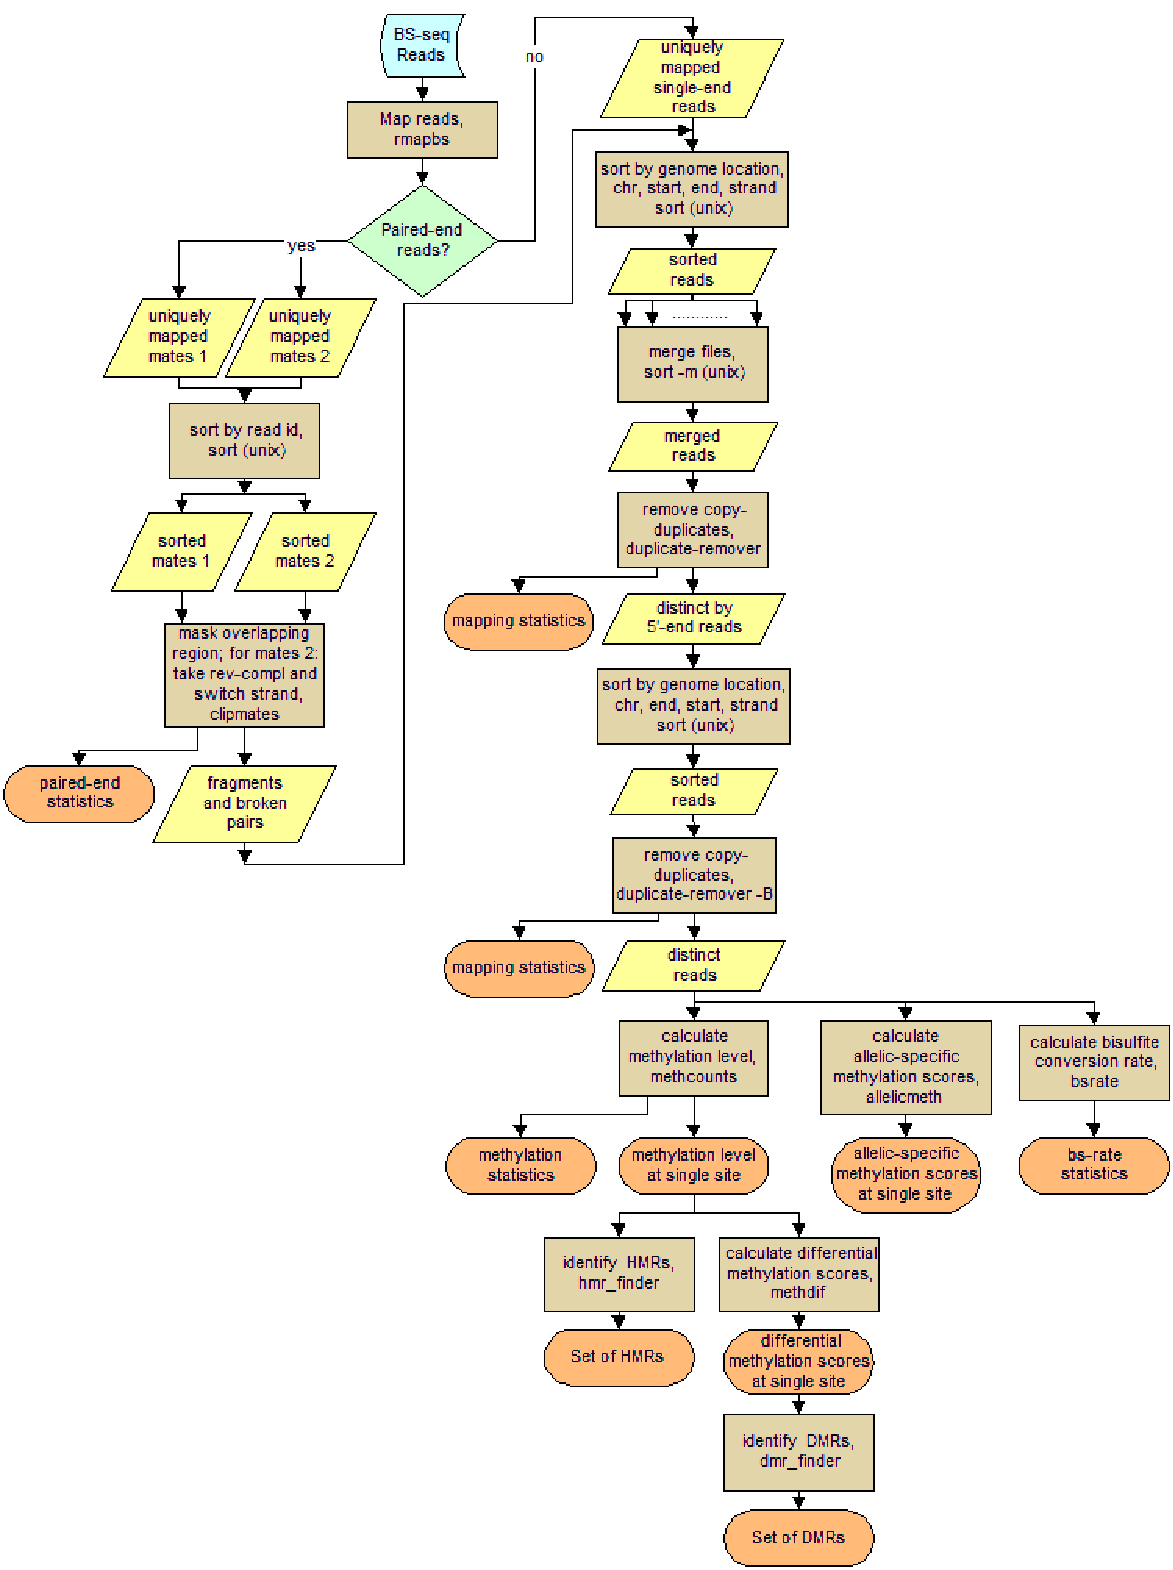
\includegraphics[width=6.3in]{figs/Methpipe_work_flow.pdf}
%   %\caption{Methpipe's Workflow}
%   %\label{fig:workflow}
% %\end{figure}

% Example data, consiting of BS-seq data from human (?) embryonic stem
% cells (ESC) and normal human foreskin fibroblasts (NHFF), has been
% provided as a tool for learning how to use the pipeline. We will refer
% to this data in the examples that illustrate each step of the pipeline
% and feel that the consistency and continuity afforded by such an
% approach will provide for the clearest learning experience. The ESC
% data consists of paired-end reads while the NHFF data consists of
% single\_end reads.

% \textbf{NOTE: I changed these file names. If these file actually exist, their names should be correspondingly changed.}\\

% The following are the three file names of the provided example
% data. These files are in FASTQ format, the format you should make sure
% your BS-seq data are in before running Methpipe on them. Two files
% belong to the ESC data set, where a "\_1" denontes the 5' end reads
% and a "\_2" denotes the 3' end reads (one file for each paired-end
% read type). The third file contains all of the single end reads of the
% NHFF data set.
% \begin{verbatim}
% Human_ESC_1.fastq, Human_ESC_2.fastq, Human_NHFF.fastq
% \end{verbatim}
% An example reference genome, to which both cell types map, is located
% in the directory \fn{hg18}. This genome is broken into 24 separate
% files (1 per chromsome), each named as \fn{chr*.fa} where \fn{*}
% denotes the chromosome number (or 'X' or 'Y' for the sex chromosomes).
% For each component of the pipeline, we complement discussion of the
% theory and purpose of each step by highlighting program options and
% input/output formats. For each of the two cell types, and example
% command will be shown for each step of Methpipe. This example command
% will only contain the basic options that are neccessary for the
% command to run.

% \section{Post-mapping processing}
% \label{sec:postmapping}

% Before mapped reads can be processed for higher level analyses,
% certain error avoiding steps must be taken. Paired mates can have
% overlapping regions, A-rich reads must be converted to T-rich reads
% through reverse complemetation, and read duplicates that are likely to
% be by-products of PCR overamplication must be excluded. The following
% sections discuss how to address each of these using Methpipe.

\subsection{Computing average methylation level in a genomic interval}
\label{sec:roimethstat}

One of the most common analysis tasks is to compute the average
methylation level through a genomic region. The \prog{roimethstat}
program accomplishes this. It takes a \prog{methcounts} output file
and a BED format file of genomic ``regions of interest'' (hence the
``roi'' in \prog{roimethstat}). It can be run as follows:
\begin{verbatim}
$ ./roimethstat -o regions_ESC_meth.bed -r regions.bed Human_ESC_Meth.bed
\end{verbatim}
The output format is also BED, and the score column now takes the
average methylation level through the interval, weighted according to
the number of reads informing about each CpG or C in the methylation
file.

\section{Creating UCSC Genome Browser tracks}
\label{sec:browser}

To view the methylation level or read coverage at individual CpG sites
in a genome browser, one needs to create a \lit{bigWig} format file
from a \fn{*\_Meth.bed} file, which is the output of \prog{methcount}
program.  A methcount file would look like this:
\begin{verbatim}
chr1	468	469	CpG:30	0.7	+
chr1	470	471	CpG:29	0.931034	+
chr1	483	484	CpG:36	0.916667	+
chr1	488	489	CpG:36	1	+
\end{verbatim}
The first 3 columns shows the physical location of each CpG sites in
the reference genome. The number in the 4th column indicates the
coverage at each CpG site. The methylation level at individual CpG
sites can be found in the 5th column. To create methylation level
tracks or read coverage tracks, one can follow these steps:
\begin{enumerate}
\item Download the \prog{wigToBigWig} program from UCSC genome
  browser's directory of binary utilities
  (\url{http://hgdownload.cse.ucsc.edu/admin/exe/}).
\item Use the \fn{fetchChromSizes} script from the same directory to
  create the \fn{*.chrom.sizes} file for the UCSC database you are
  working with (e.g. hg18). Note that this is the file that is
  referred to as \fn{hg18.chrom.sizes} in step 3.
\item To create a \fn{bw} track for methylation level at single CpG
  sites, modify and use the following command:
\begin{verbatim}
$ cut -f 1-3,5 Human_ESC_Meth.bed | \
     wigToBigWig /dev/stdin hg18.chrom.sizes Human_ESC_Meth.bw
\end{verbatim}
  To create a \fn{bw} track for coverage at single CpG sites, modify
  and use the following command:
\begin{verbatim}
$ tr ':' 'Ctrl+v Tab' < Human_ESC_Meth.bed | cut -f 1-3,5 | \
     wigToBigWig /dev/stdin hg18.chrom.sizes Human_ESC_Reads.bw
\end{verbatim}
\end{enumerate}

\noindent
You might also want to create \fn{bidBed} browser tracks for HMRs,
AMRs or DMRs. To do so, follow these steps:
\begin{enumerate}
\item Download the \prog{bedToBigBed} program from the UCSC Genome
  Browser directory of binary utilities
  (\url{http://hgdownload.cse.ucsc.edu/admin/exe/}).
\item Use the \fn{fetchChromSizes} script from the same directory to
  create the \fn{*.chrom.sizes} file for the UCSC database you are
  working with (e.g. hg18). Note that this is the file that is
  referred to as \fn{hg18.chrom.sizes} in step 3.
\item Modify and use the following comands: For \fn{*\_HMR.bed} files
  with non-integer score in their 5th column, one needs to round the
  score to integer value, for example:
\begin{verbatim}
$ awk -v OFS="\t" '{print $1, $2, $3, $4, int($5), $6}' \
      Human_ESC_HMR.bed > Human_ESC_HMR.bed.tmp
$ bedToBigBed Human_ESC_HMR.bed.tmp hg18.chrom.sizes Human_ESC_HMR.bb
\end{verbatim}
Otherwise, one can run the following command directly.
\begin{verbatim}
$ bedToBigBed Human_ESC_HMR.bed hg18.chrom.sizes Human_ESC_HMR.bb
\end{verbatim}
\end{enumerate}

\end{document}
